\documentclass[aspectratio=169]{beamer}
\usetheme{Madrid}

\usepackage[T1]{fontenc}
\usepackage{lmodern}
\usepackage{pifont}
\usepackage{amsmath}
\usepackage{amssymb}
\usepackage{nicefrac}
\usepackage{comment}
\usepackage{multicol}
\usepackage{siunitx}
\sisetup{
  per-mode=fraction,
  fraction-function=\nicefrac,
  detect-weight=true,
  detect-family=true
}

\usepackage{colortbl}
\usepackage{xcolor}
\usepackage{fontawesome5}
\usepackage{pifont}
\newcommand{\cmark}{\ding{51}} % ✓
\newcommand{\xmark}{\ding{55}} % ✗

\usepackage[yyyymmdd]{datetime}
\usepackage{tikz}
\usepackage{circuitikz}
\usepackage{pgfplots}

\usepackage{hyperref}
\usepackage{mathtools}
\usepackage{adjustbox}
\usepackage{array}
\newcolumntype{C}[1]{>{\centering\arraybackslash}p{#1}}

\usepackage{animate}
%\usepackage{cite}

\usepackage[style=alphabetic,backend=biber, style=numeric, sorting=none]{biblatex}
%\addbibresource{references.bib}
\renewcommand*{\mkbibacro}[1]{#1}

\usetikzlibrary{arrows, shapes, calc, positioning}
%\usetikzlibrary{external}
%\usepgfplotslibrary{external}
%\tikzexternalize
\pgfplotsset{compat=1.18}

\renewcommand{\dateseparator}{--}

\makeatletter
\let\slideno\beamer@slideinframe
\makeatother


\DeclarePairedDelimiter\bra{\langle}{\rvert}
\DeclarePairedDelimiter\ket{\lvert}{\rangle}
\DeclarePairedDelimiterX\braket[2]{\langle}{\rangle}{#1\,\delimsize\vert\,\mathopen{}#2}

\definecolor{links}{HTML}{2A1B81}
\hypersetup{colorlinks,linkcolor=,urlcolor=links}

\definecolor{UDSgreenDurable}{RGB}{149, 193, 78}
\definecolor{UDSgreenVivacite}{RGB}{121, 181, 81}
\definecolor{UDSgreenCreativite}{RGB}{90, 173, 85}
\definecolor{UDSgreenFierte}{RGB}{0, 167, 89}
\definecolor{UDSgreenSolidarite}{RGB}{61, 143, 88}
\definecolor{UDSgreenBien-etre}{RGB}{68, 124, 90}
\definecolor{UDSgreenReussite}{RGB}{72, 106, 92} 
\definecolor{UDSgrey}{RGB}{228, 232, 225} 

\setbeamercolor{palette primary}{bg=UDSgreenSolidarite,fg=white}
\setbeamercolor{palette secondary}{bg=UDSgreenFierte,fg=white}
\setbeamercolor{palette tertiary}{bg=UDSgreenCreativite,fg=white}
\setbeamercolor{palette quaternary}{bg=UDSgreenReussite,fg=white}
\setbeamercolor{structure}{fg=UDSgreenReussite} % itemize, enumerate, etc
\setbeamercolor{section in toc}{fg=UDSgreenBien-etre} % TOC sections
\setbeamercolor{background canvas}{bg=UDSgrey}


\setbeamertemplate{caption}[numbered]


\makeatletter
\newcommand\titlegraphicii[1]{\def\inserttitlegraphicii{#1}}
\titlegraphicii{}
\setbeamertemplate{title page}
{
    {\usebeamercolor[fg]{titlegraphic}\inserttitlegraphic\hfill\inserttitlegraphicii\par}
    \begin{multicols}{2}
        \begin{beamercolorbox}[sep=8pt,center,shadow=true,rounded=true, wd=0.5\textwidth]{title}
            \usebeamerfont{title}\inserttitle\par%
            {\usebeamerfont{subtitle}\usebeamercolor[fg]{subtitle}\insertsubtitle\par}%
            {\vspace{24pt}\small\usebeamerfont{author}\insertauthor\par}%
        \end{beamercolorbox}%
    \vfill\null
    \columnbreak
    \end{multicols}
}
\makeatother
\author{Pascal-Emmanuel Lachance}
\title{PPPPP03}
\subtitle{Comment conçevoir un\\ Power Delivery Network?}
\institute{Compétitions de Conception de Circuits Imprimés}
\date{\today}
\titlegraphic{
\includegraphics[scale = 0.3]{pictures/logo/udes_logo.pdf}}
%\titlegraphicii{
\includegraphics[scale = 0.2]{pictures/logo/3IT_logo.png}}
%\logo{
\includegraphics[scale = 0.15]{pictures/logo/udes_logo.pdf}}

\defbeamertemplate*{footline}{mytheme}
{
    \leavevmode%
    \hbox{%
    \begin{beamercolorbox}[wd=.33\paperwidth,ht=2.25ex,dp=1ex,center]{author in head/foot}%
        \usebeamerfont{author in head/foot} Pascal-Emmanuel Lachance
    \end{beamercolorbox}%
    \begin{beamercolorbox}[wd=.34\paperwidth,ht=2.25ex,dp=1ex,center]{title in head/foot}%
        \usebeamerfont{title in head/foot}\inserttitle
    \end{beamercolorbox}}%
    \begin{beamercolorbox}[wd=.33\paperwidth,ht=2.25ex,dp=1ex,right]{date in head/foot}%
        \hfill\usebeamerfont{date in head/foot}\today{}
        \hfill%\hspace*{2em}
        \insertframenumber{} / \inserttotalframenumber\hspace*{2ex} 
    \end{beamercolorbox}
}%

\defbeamertemplate*{frametitle}{mytheme}
{%
    \vspace{0cm}
    {\usebeamerfont{title}\usebeamercolor[bg]{title}\insertframetitle}
    \par
    \vspace{-0.55cm}
    \hfill
    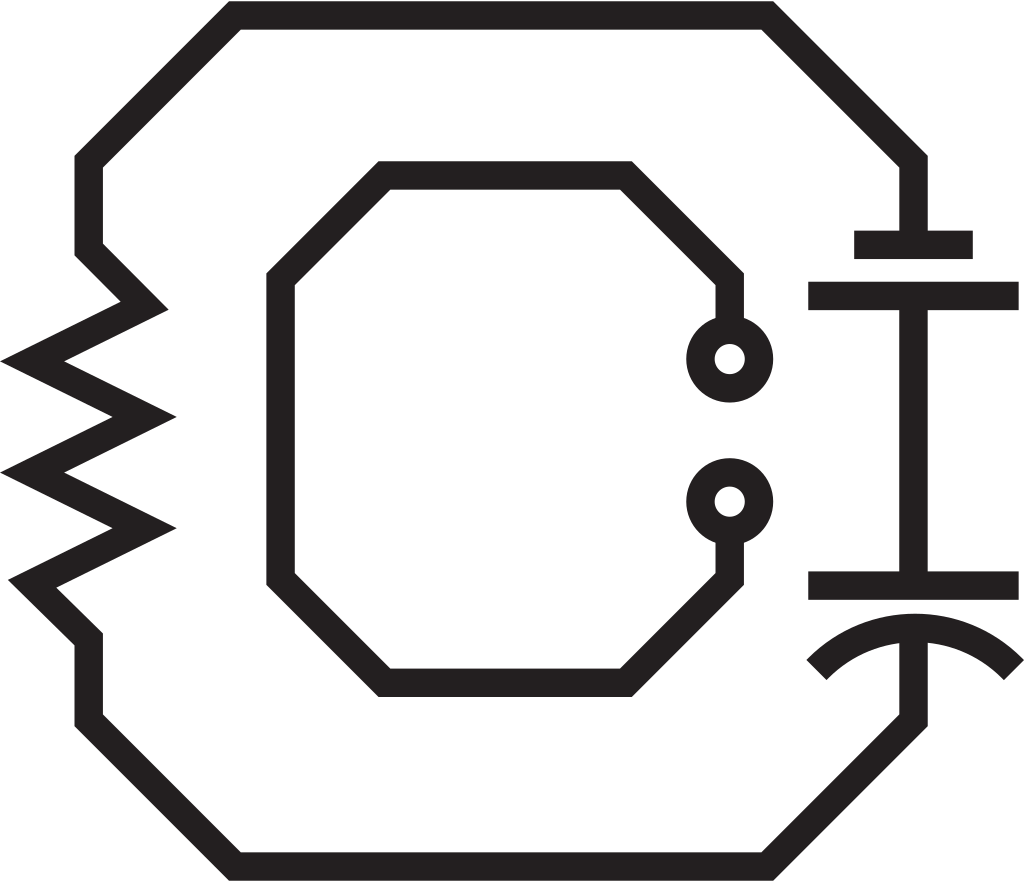
\includegraphics[height=0.635cm]{pictures/logo/c3i.png}
    
\includegraphics[height=0.635cm]{pictures/logo/m1_alpha.pdf}
    \par
    \vspace{-0.3cm}
    \textcolor{UDSgreenSolidarite}{\noindent\rule{\textwidth}{1pt}}
}%

\setbeamertemplate{itemize item}{\large$\bullet$}
\setbeamertemplate{itemize subitem}{\small$\bullet$}
\setbeamertemplate{itemize subsubitem}{\tiny$\bullet$}
\usebeamertemplate{mytheme}

\newif\ifINTRO
\INTROfalse

\ifINTRO
    \includeonlyframes{intro}
    \setbeamertemplate{navigation symbols}{}
\fi



% ----------------------- BEGIN DOCUMENT ------------------------

\begin{document}

\usebackgroundtemplate{
\begin{tikzpicture}[remember picture, overlay]
        \node[at=(current page.center)] {
            {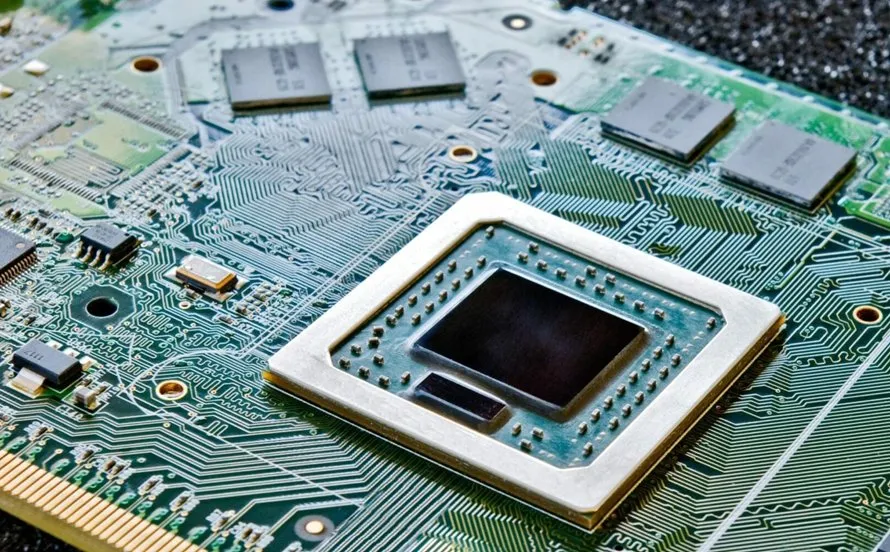
\includegraphics[width=\paperwidth,keepaspectratio]{pictures/background/background-PCB.png}}
        };
    \end{tikzpicture}
}

\begin{frame}[plain]
    \maketitle
\end{frame}

\usebackgroundtemplate{
\begin{tikzpicture}[remember picture, overlay]
        \node[at=(current page.center)] {
            {
\includegraphics[width=\paperwidth,keepaspectratio]{pictures/background/background-pcb-poster.png}}
        };
    \end{tikzpicture}
}

\begin{frame}[plain, label=intro]
    \centering
    \Large

    \textcolor{white}{
        \LARGE{\textbf{\inserttitle}}\\
        \textbf{\textit{\insertsubtitle}}\\
        Par: \insertauthor\\
    }
    \vspace{24pt}
    \begin{tabular}{c l}
        \textcolor{UDSgreenFierte}{\faShield*}
            & \textcolor{white}{~Comment protéger une alimentation?}\\
            [0.3em]
        \textcolor{UDSgreenFierte}{\faSlidersH}
            & \textcolor{white}{~Quels sont les types de régulateurs?}\\
            [0.3em]
        \textcolor{UDSgreenFierte}{\faEquals}
            & \textcolor{white}{~À quoi sert le découplage?}\\
            [0.3em]
        \textcolor{UDSgreenFierte}{\faWaveSquare}
            & \textcolor{white}{~Comment filtrer une alimentation?}\\
            [0.3em]
        \textcolor{UDSgreenFierte}{\faProjectDiagram}
            & \textcolor{white}{~Comment conçevoir un arbre d'alimentation?}\\
    \end{tabular}
\end{frame}



% - TOC -
\usebackgroundtemplate{
\begin{tikzpicture}[remember picture, overlay]
        \node[at=(current page.center)] {
            
\includegraphics[width=\paperwidth, keepaspectratio]{pictures/background/background3.jpg}
        };
    \end{tikzpicture}
}


\AtBeginSection[]{
    \begin{frame}[plain]
         \vfill
         \centering
         \begin{beamercolorbox}[sep=6pt,center,shadow=true,rounded=true]{title}
             \usebeamerfont{title}\insertsectionhead\par%
         \end{beamercolorbox}
         \tableofcontents[currentsection,hideothersubsections]
         \vfill
  \end{frame}
}

\AtBeginSubsection[]
{
    \begin{frame}[plain]
         \vfill
         \centering
         \begin{beamercolorbox}[sep=6pt,center,shadow=true,rounded=true]{title}
             \usebeamerfont{title}\insertsectionhead\par%
         \end{beamercolorbox}
         \tableofcontents[currentsection,currentsubsection,subsectionstyle=show/shaded/hide]
         \vfill
    \end{frame}
}



% ------------ SECTIONS -----------

%!TEX root = ../main.tex 

\section{Comment protéger une alimentation?}

%!TEX root = ../main.tex 

\section{Quels sont les types de régulateurs?}

\subsection{Régulateurs Linéaires}
\subsection{Régulateurs \textit{Switching}}
%!TEX root = ../main.tex 

\section{Comment filtrer une alimentation?}

\subsection{Pourquoi filtrer une alimentation?}

\begin{frame}{Pourquoi Filtrer?}
    \begin{columns}
        \begin{column}{0.5\textwidth}
            \begin{center}
                \textbf{Signal Integrity}
            \end{center}
        \end{column}
        \begin{column}{0.5\textwidth}
            \begin{center}
                \textbf{Electromagnetic Interference}
            \end{center}
        \end{column}
    \end{columns}
    \begin{columns}
        \begin{column}{0.5\textwidth}
            \begin{itemize}
                \item Signaux Clean
                \item Marges d'opérations respectées
            \end{itemize}

            \centering
            \begin{tabular}{c l}
                \textcolor{UDSgreenFierte}{\faUndo}   & Rélections \\
                \textcolor{UDSgreenFierte}{\faExchange*}         & Crosstalk \\
                \textcolor{UDSgreenFierte}{\faCompress}     & Ground Bounce \\
                \textcolor{UDSgreenFierte}{\faFilter}   & \textbf{Filtration de Power} \\
            \end{tabular}
        \end{column}
        \begin{column}{0.5\textwidth}
            \begin{itemize}
                \item Passer les tests EMC
                \item Ne pas influencer d'autres circuits
                \begin{itemize}
                    \item Émissions
                    \item Immunité au bruit
                \end{itemize}

                \centering
                \begin{tabular}{c l}
                    \textcolor{UDSgreenFierte}{\faPuzzlePiece}   & Layout \\
                    \textcolor{UDSgreenFierte}{\faArrowDown}         & Grounding \\
                    \textcolor{UDSgreenFierte}{\faShield*}     & Shielding \\
                    \textcolor{UDSgreenFierte}{\faFilter}   & \textbf{Filtration de Power} \\
                \end{tabular}
            \end{itemize}
        \end{column}
    \end{columns}
\end{frame}

\begin{frame}{But d'un filtre sur l'alimentation}
    \begin{itemize}
        \item \textbf{Le but d'un filtre est de fournir le chemin de plus faible impédance vers le ground aux signaux haute-fréquence}.
        \bigskip
        \item \textbf{Le but d'un filtre est de contrôler la propagation du bruit sur l'alimentation.}
    \end{itemize}
\end{frame}

\begin{frame}{Filtration de Power}
    \begin{itemize}
        \item Tout commence avec le power
        \item Le PDN devrait constituer 25\% à 50\% de la difficulté d'un projet
        \bigskip
        \item Plein de façon de filtrer
        \item Réduire le bruit sur l'alimentation
        \item Avoir une alimentation purement DC
        \bigskip
        \item<2-> Jouer avec les impédances de mon alimentation
        \begin{itemize}
            \item<2->[] \textcolor{UDSgreenFierte}{\faEquals} ~Découplage 
            \item<2->[] \textcolor{UDSgreenFierte}{\faSync} ~Rajouter des inductances
            \item<2->[] \textcolor{UDSgreenFierte}{\faPuzzlePiece} ~Faire attention à son layout 
        \end{itemize}
        \item<2-> Ajouter des composantes actives
        \begin{itemize}
            \item<2->[] \textcolor{UDSgreenFierte}{\faRulerHorizontal} ~Régulateurs Linéaires
        \end{itemize}
    \end{itemize}
\end{frame}

\begin{frame}{D'où provient le bruit}
    \Large
    \centering
    \begin{tabular}{c l}
        \textcolor{UDSgreenFierte}{\faWaveSquare}
            & IC qui toggle \\
        [0.6em]
        \textcolor{UDSgreenFierte}{\faRoute}
            & Longues lignes de transmission \\
        \hspace{18pt}\textcolor{UDSgreenFierte}{\faExchange*}
            & \hspace{18pt}Crosstalk \\
        \hspace{18pt}\textcolor{UDSgreenFierte}{\faBroadcastTower}
            & \hspace{18pt}Antennes \\
        [0.6em]
        \textcolor{UDSgreenFierte}{\faProjectDiagram} 
            & Mauvais chemins de retour \\
        \hspace{18pt}\textcolor{UDSgreenFierte}{\faExchange*}
            & \hspace{18pt}Crosstalk \\
        \hspace{18pt}\textcolor{UDSgreenFierte}{\faStumbleupon}
            & \hspace{18pt}Ground Bounce \\
        \hspace{18pt}\textcolor{UDSgreenFierte}{\faBroadcastTower}
            & \hspace{18pt}Antennes
    \end{tabular}
\end{frame}



\subsection{Démonstration}

\subsection{Filtrer l'entrée}
\begin{frame}{L'entrée d'un système d'alimentation}
    \begin{columns}
        \begin{column}{0.66\textwidth}
            \begin{itemize}
                \item[] \textcolor{UDSgreenFierte}{\faRoute} 
                    ~Long fil qui provient d'une Power Supply
                \item[] \textcolor{UDSgreenFierte}{\faSync} 
                    ~Inductance Parasite
                \bigskip
                \item[] \textcolor{UDSgreenFierte}{\faSatelliteDish}
                    ~Pick-Up du bruit extérieur 
                \item[] \textcolor{UDSgreenFierte}{\faSignature}
                    ~Signal potentiellement bruité
                \bigskip
                \item[] \textcolor{UDSgreenFierte}{\faLongArrowAltRight}
                \textbf{~Demande de courant au travers d'une bobine.}
                \item[] \textcolor{UDSgreenFierte}{\faWaveSquare}
                \textbf{~Demande de courant non-constante}
            \end{itemize}
        \end{column}
        \begin{column}{0.33\textwidth}
            \begin{figure}
                \centering
                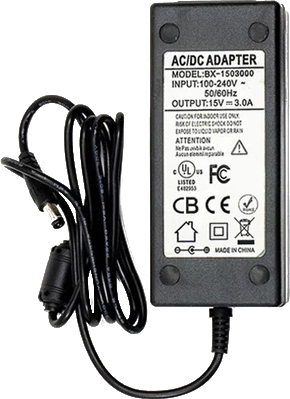
\includegraphics[width=\textwidth]{pictures/power-brick.png}
            \end{figure}
        \end{column}
    \end{columns}
\end{frame}

\begin{frame}{Découplage}
    \begin{itemize}
        \item $X_L \propto -X_C$
        \item Rajouter de la capacitance pour compenser l'inductance
        \item Plus ton fil est long, plus tu veux de capacitance
        \item Le power devrait provenir des condensateurs
        \item \textit{Couper le chemin d'inductance}
    \end{itemize}

    \pause
    \vfill
    \begin{center}
    \resizebox{0.8\textwidth}{!}{
    \ctikzset{bipoles/cuteinductor/height=0.15}
    \ctikzset{bipoles/cuteinductor/width=0.5}
    \begin{circuitikz}[american voltages]
        \draw [thick]
        (0, 0) to [short, *-] (10, 0)
        to [european resistor, l_=${LOAD}$] (10, 4)
        (0, 0) to [open, v<=$V$] (0, 4)
        to [american inductor, l=$wire$, color=red] (5, 4)
        to [short] (6, 4)
        to [cute inductor, l=$pcb$, color=UDSgreenFierte] (10, 4)
        ;

        \draw [thick] (5, 0) to [C, l=$bulk$, color=red] (5, 4);
        \draw [thick] (6, 0) to [C, l_=$decoupling$, color=UDSgreenFierte] (6, 4);

        \draw[->, thick, red]
        (1, 3.5) to [out=0, in=180] (3.5, 3.5)
        to [out=0, in=90] (4.5, 2.5);
        \draw[->, thick, UDSgreenFierte]
        (6.5, 2.5) to [out=90, in=180] (7.5, 3.5)
        to [out=0, in=180] (8.5, 3.5)
        to [out=0, in=90] (9.5, 2.5);
    \end{circuitikz}
    }
    \end{center}
\end{frame}

\begin{frame}{Filtrage avancé d'une entrée d'alimentation}
    \begin{itemize}
        \item Découplage permet de fournir un chemin de faible impédance aux signaux haute-vitesse
        \item Bulk permet d'emmagasiner des charges et que le power provienne des condensateurs et non du fil
        \bigskip
        \item<2-> \textbf{Contrôler la propagation du bruit}
        \begin{itemize}
            \item<2->[] \textcolor{UDSgreenFierte}{\faArrowRight} ~Limiter le bruit au board
            \item<2->[] \textcolor{UDSgreenFierte}{\faArrowLeft} ~Limiter le bruit hors du board
            \item<2->[] \textcolor{UDSgreenFierte}{\faFileContract} ~Passer EMC
        \end{itemize}
    \end{itemize}
\end{frame}

\begin{frame}{Rajouter des inductances}
    \begin{itemize}
        \item Rajouter de l'inductance permet de bien contrôler où va le bruit haute-fréquence.
        \item $X_L = 2\pi fL$
        \item Si $X_L > X_C$, le bruit va passer par $X_C$.
        \bigskip
        \item On vient de passer tout ce temps pour compenser l'inductance du fil d'alimentation
        \item<2-> Maintenant, on contrôle l'inductance!
        \begin{itemize}
            \item<2-> Les condensateurs de découplage fournissent la puissance haute fréquence
            \item<2-> Les condensateurs de bulk fournissent la puissance basse fréquence
            \item<2-> Les condensateurs de bulk rechargent les condensateurs de découplage
            \item<2-> L'alimentation fournit du power DC pour recharger les condensateurs de bulk
        \end{itemize}
    \end{itemize}
\end{frame}


\subsection{Filtrer la sortie d'un régulateur}
\subsection{Filtrer au IC}
%!TEX root = ../main.tex 

\section{Comment conçevoir un arbre d'alimentation?}

\subsection{Déterminer les besoins}

\begin{frame}{Tensions d'opération}
    \begin{itemize}
        \item Chaque puce a une tension d'opération
        \item Parfois plusieurs tensions possible ($\SI{3.3}{\volt}$ jusqu'à $\SI{5}{\volt}$)
        \item Parfois plusieurs tensions nécessaires!
        \bigskip
        \item Parfois les puces peuvent avoir des IO à des tensions différentes
    \end{itemize}
\end{frame}

\begin{frame}{Courant d'opération}
    \begin{columns}
        \only<2> {
            \begin{column}{0.55\textwidth}
        }
        \only<1, 3> {
            \begin{column}{0.66\textwidth}
        }
            \begin{itemize}
                \item Pour chaque puce, à sa tension d'opération, récupérer:
                \begin{itemize}
                    \item Le courant minimal (sleep)
                    \item Le courant normal d'opération
                    \item Le courant maximal d'opération
                \end{itemize}
                \item Parfois tout le même
                \only<2-> {
                    \bigskip
                    \item Conçevoir circuit pour pouvoir passer le courant maximal
                    \item Choisir régulateurs pour avoir efficacité maximale au courant nominal
                }
                \only<3> {
                    \bigskip
                    \item Aussi rassembler tous les courants autres
                    \begin{itemize}
                        \item Moteurs
                        \item LEDs et affichage
                        \item Connecteurs et sous-cartes
                    \end{itemize}
                }
            \end{itemize}
        \end{column}
        
        \only<2> {
        \begin{column}{0.45\textwidth}
            \begin{figure}
                \includegraphics<2>[width=\textwidth, height=0.75\textheight, keepaspectratio]{pictures/switching-efficiency-curve.png}
            \end{figure}
        \end{column}
        }
        \only<1, 3> {
        \begin{column}{0.33\textwidth}
            \begin{figure}
                \includegraphics<3>[width=\textwidth, height=0.75\textheight, keepaspectratio]{pictures/switching-efficiency-curve.png}
            \end{figure}
        \end{column}
        }
    \end{columns}
\end{frame}

\begin{frame}{Trouver le courant d'opération}
    \begin{figure}
        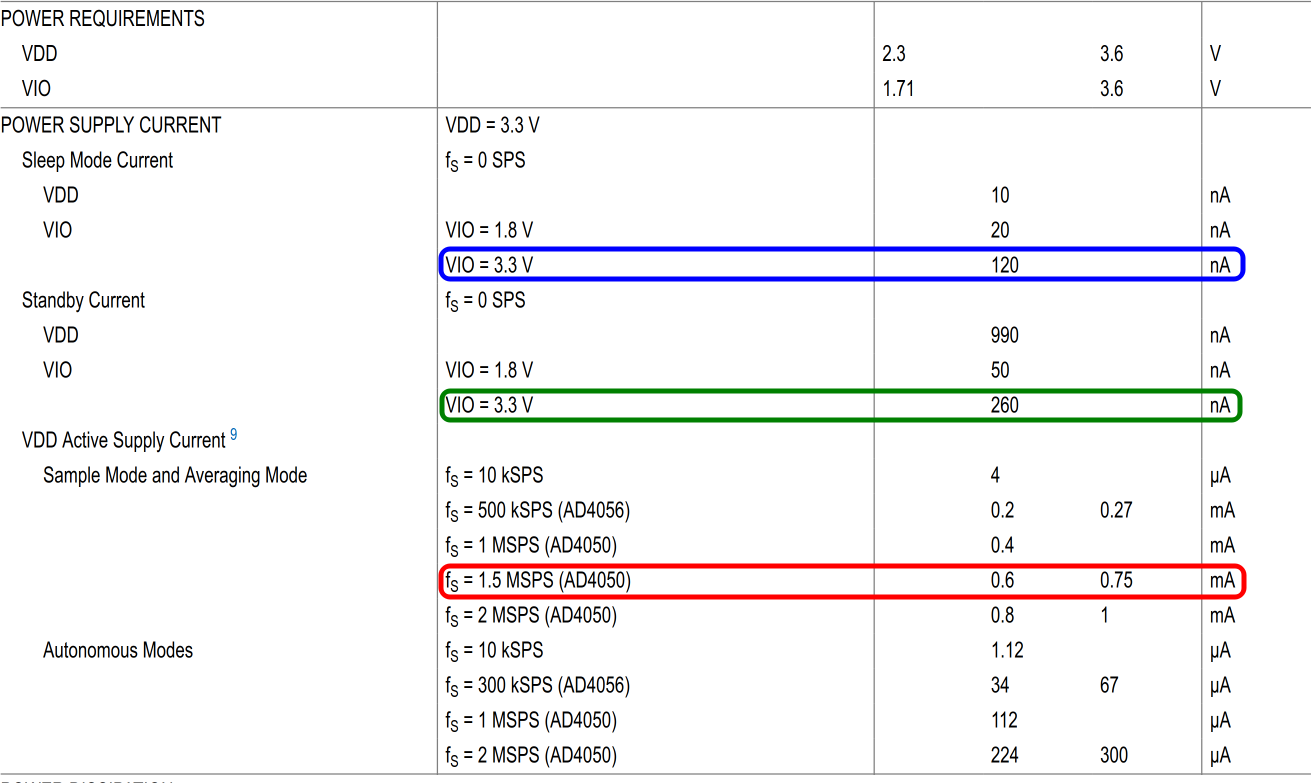
\includegraphics[width=\textwidth, height=0.75\textheight, keepaspectratio]{pictures/ad4050-power.png}
    \end{figure}
    \href{https://www.analog.com/media/en/technical-documentation/data-sheets/ad4050-ad4056.pdf}{Analog Devices - AD4050 - 12-Bit 2MSPS SAR ADC}
\end{frame}

\begin{frame}{Besoins en stabilité}
    \begin{itemize}
        \item Déterminer les besoins de chaque puce en stabilité
        \item Quel est le $\Delta V$ maximum tolérable pour l'opération de la puce
        \item Quelle est la précision nécessaire pour une puce analogique
        \item À quel point un $\Delta V$ peut introduire un $\Delta f$ pour la fréquence?
    \end{itemize}

    \begin{columns}
        \begin{column}{0.5\textwidth}
            \only<2-> {
            \begin{itemize}
                \item Toujours mieux de quantifier
                \item \textbf{Permet de déterminer type de régulateur}
            \end{itemize}
            }
        \end{column}
        \begin{column}{0.5\textwidth}
            \begin{figure}
                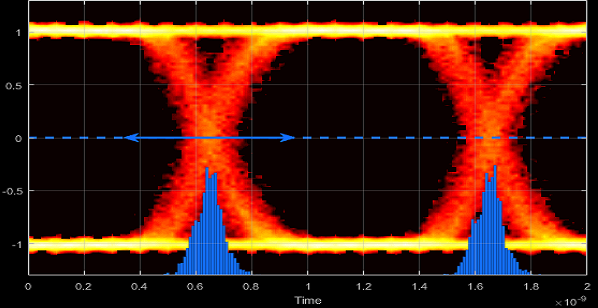
\includegraphics[width=\textwidth, height=0.45\textheight, keepaspectratio]{pictures/eye-diagram.png}
            \end{figure}
        \end{column}
    \end{columns}
\end{frame}


\subsection{Bilan d'alimentation}

\begin{frame}{Bilan d'alimentation - Example - Alimentation 12V}
    \centering
    \Large
    \renewcommand{\arraystretch}{1.2}
    \vspace{-6pt}

    \begin{tabular}{>{\color{UDSgreenSolidarite}}c l | l | l | l | l | l}
    \rowcolor{UDSgreenSolidarite}
    & \textcolor{white}{\textbf{IC}}
    & \textcolor{white}{\textbf{Tension}}
    & \textcolor{white}{\textbf{I min}}
    & \textcolor{white}{\textbf{I nom}}
    & \textcolor{white}{\textbf{I max}} 
    & \textcolor{white}{\textbf{Type}}\\
    \hline
    \textcolor{UDSgreenFierte}{\faMicrochip} &
        \textbf{IC 1} &
        $\SI{3.3}{\volt}$ &
        $\SI{10}{\micro\ampere}$ &
        $\SI{17.5}{\milli\ampere}$ &
        $\SI{17.5}{\milli\ampere}$ &
        Digital\\
    \textcolor{UDSgreenFierte}{\faMicrochip} &
        \textbf{IC 2} &
        $\SI{3.3}{\volt}$ &
        $\SI{10}{\milli\ampere}$ &
        $\SI{10}{\milli\ampere}$ &
        $\SI{10}{\milli\ampere}$ &
        Digital\\
    & \hspace{16pt}\raisebox{10pt}{\rotatebox{-90}{\faLevelUp*}} &
        $\SI{3.3}{\volt}$ &
        $\SI{0}{\micro\ampere}$ &
        $\SI{10}{\milli\ampere}$ &
        $\SI{50}{\milli\ampere}$ &
        Analog\\
    \textcolor{UDSgreenFierte}{\faMicrochip} &
        \textbf{IC 3} &
        $\SI{2.5}{\volt}$ &
        $\SI{20}{\milli\ampere}$ &
        $\SI{20}{\milli\ampere}$ &
        $\SI{50}{\milli\ampere}$ &
        Analog\\
    \textcolor{UDSgreenFierte}{\faLightbulb} &
        \textbf{LEDs} &
        $\SI{5}{\volt}$ &
        $\SI{0}{\ampere}$ &
        $\SI{80}{\milli\ampere}$ &
        $\SI{80}{\milli\ampere}$ &
        Digital\\
    \textcolor{UDSgreenFierte}{\faUsb} &
        \textbf{USB} &
        $\SI{5}{\volt}$ &
        $\SI{0}{\ampere}$ &
        $\SI{100}{\milli\ampere}$ &
        $\SI{500}{\milli\ampere}$ &
        Digital\\
    \textcolor{UDSgreenFierte}{\faFan} &
        \textbf{Stepper} &
        $\SI{12}{\volt}$ &
        $\SI{0}{\ampere}$ &
        $\SI{300}{\milli\ampere}$ &
        $\SI{750}{\milli\ampere}$ &
        Digital\\
    \hline
    \textcolor{UDSgreenFierte}{\boldmath$\Sigma$} & \textbf{Total} & &
        \textbf{\boldmath$\SI{30.01}{\milli\ampere}$} &
        \textbf{\boldmath$\SI{537.5}{\milli\ampere}$} &
        \textbf{\boldmath$\SI{1457.5}{\milli\ampere}$} & \\
    \end{tabular}
\end{frame}

\begin{frame}{Bilan d'alimentation - Example - Alimentation 12V}
    \centering
    \Large
    \renewcommand{\arraystretch}{1.2}
    \vspace{-6pt}

    \begin{tabular}{>{\color{UDSgreenSolidarite}}c l | l | l | l}
    \rowcolor{UDSgreenSolidarite}
    & \textcolor{white}{\textbf{IC}}
    & \textcolor{white}{\textbf{Tension}}
    & \textcolor{white}{\textbf{I max}} 
    & \textcolor{white}{\textbf{Type}}\\
    \hline
    \textcolor{UDSgreenFierte}{\faMicrochip} &
        \textbf{IC 1} &
        $\SI{3.3}{\volt}$ &
        $\SI{17.5}{\milli\ampere}$ &
        Digital\\
    \textcolor{UDSgreenFierte}{\faMicrochip} &
        \textbf{IC 2} &
        $\SI{3.3}{\volt}$ &
        $\SI{10}{\milli\ampere}$ &
        Digital\\
    & \hspace{16pt}\raisebox{10pt}{\rotatebox{-90}{\faLevelUp*}} &
        $\SI{3.3}{\volt}$ &
        $\SI{50}{\milli\ampere}$ &
        Analog\\
    \textcolor{UDSgreenFierte}{\faMicrochip} &
        \textbf{IC 3} &
        $\SI{2.5}{\volt}$ &
        $\SI{50}{\milli\ampere}$ &
        Analog\\
    \textcolor{UDSgreenFierte}{\faLightbulb} &
        \textbf{LEDs} &
        $\SI{5}{\volt}$ &
        $\SI{80}{\milli\ampere}$ &
        Digital\\
    \textcolor{UDSgreenFierte}{\faUsb} &
        \textbf{USB} &
        $\SI{5}{\volt}$ &
        $\SI{500}{\milli\ampere}$ &
        Digital\\
    \textcolor{UDSgreenFierte}{\faFan} &
        \textbf{Stepper} &
        $\SI{12}{\volt}$ &
        $\SI{750}{\milli\ampere}$ &
        Digital\\
    \hline
    \textcolor{UDSgreenFierte}{\boldmath$\Sigma$} & \textbf{Total} & &
        \textbf{\boldmath$\SI{1457.5}{\milli\ampere}$} & \\
    \end{tabular}
\end{frame}

\begin{frame}{Diagramme d'alimentation}
    \centering
    \resizebox{\textwidth}{!}{
    \begin{tikzpicture}[
        block/.style = {rectangle, draw,
        minimum height=0.75cm,
        minimum width=2cm,
        align=center,
        very thick,
        rounded corners=0.1cm},
        node distance=0.8cm and 0.6cm,
        >={Stealth[round]},
        x = 3cm,
        y = 1cm
    ]

    \node(inlabel) at (0, 0) {};

    \node[block] (prot) at (0.5, 0)
        {\textcolor{UDSgreenFierte}{\faShield*} ~\textcolor{black}{Protections}};
    \node[block] (step) at (5,   0)
        {\textcolor{UDSgreenFierte}{\faFan} ~\textcolor{black}{Stepper}};
    \node[block] (5v)   at (2,  -1)
        {\textcolor{UDSgreenFierte}{\faWaveSquare} ~\textcolor{black}{\SI{5}{\volt}}};
    \node[block] (led)  at (5,  -1)
        {\textcolor{UDSgreenFierte}{\faLightbulb} ~\textcolor{black}{LED}};
    \node[block] (usb)  at (5,  -2)
        {\textcolor{UDSgreenFierte}{\faUsb} ~\textcolor{black}{USB}};
    \node[block] (3v3)  at (2,  -3)
        {\textcolor{UDSgreenFierte}{\faWaveSquare} ~\textcolor{black}{\SI{3.3}{\volt}}};

    \node[block] (3v3a) at (3.33,  -5)
        {\textcolor{UDSgreenFierte}{\faSync} ~\textcolor{black}{Ferrite}};
    \node[block] (3v3ic1) at (3.33,  -3)
        {\textcolor{UDSgreenFierte}{\faSync} ~\textcolor{black}{Ferrite}};
    \node[block] (3v3ic2) at (3.33,  -4)
        {\textcolor{UDSgreenFierte}{\faSync} ~\textcolor{black}{Ferrite}};

    \node[block] (ic1)  at (5,  -3)
        {\textcolor{UDSgreenFierte}{\faMicrochip} ~\textcolor{black}{IC 1}};
    \node[block] (ic2)  at (5,  -4)
        {\textcolor{UDSgreenFierte}{\faMicrochip} ~\textcolor{black}{IC 2}};
    \node[block] (ic2a) at (5,  -5)
        {\textcolor{UDSgreenFierte}{\faMicrochip} ~\textcolor{black}{IC 2A}};
    \node[block] (2v5)  at (3.33,  -6)
        {\textcolor{UDSgreenFierte}{\faLongArrowAltRight} ~\textcolor{black}{\SI{2.5}{\volt}}};
    \node[block] (ic3)  at (5,  -6)
        {\textcolor{UDSgreenFierte}{\faMicrochip} ~\textcolor{black}{IC 3}};

    \draw[->, ultra thick, color=red]
         ($(inlabel)+(-1.25, 0)$) -- (prot.west)
         node[midway, above]
         {\textcolor{black}{Input $\SI{12}{\volt}$}};

    \draw[->, ultra thick, color=red]
         (prot) -- (step)
         node[midway, above]
         {\textcolor{black}{$\SI{750}{\milli\ampere}$}};
    \draw[->, ultra thick, color=red]
         (prot) |- (5v)
         node[pos=0.75, above]
         {\textcolor{black}{$?\SI{}{\milli\ampere}$}};
    \draw[->, ultra thick, color=red]
         (prot) |- (3v3)
         node[pos=0.75, above]
         {\textcolor{black}{$?\SI{}{\milli\ampere}$}};

    \draw[->, ultra thick, color=magenta]
         (5v) -- (led)
         node[midway, above]
         {\textcolor{black}{$\SI{80}{\milli\ampere}$}};
    \draw[->, ultra thick, color=magenta]
         (5v) |- (usb)
         node[pos=0.79, above]
         {\textcolor{black}{$\SI{500}{\milli\ampere}$}};

    \draw[->, ultra thick, color=blue]
         (3v3) -- (3v3ic1)
         node[midway, above]
         {\textcolor{black}{$\SI{17.5}{\milli\ampere}$}};
    \draw[->, ultra thick, color=blue]
         (3v3ic1) -- (ic1)
         node[midway, above]
         {\textcolor{black}{$\SI{17.5}{\milli\ampere}$}};
    \draw[->, ultra thick, color=blue]
         (3v3) |- (3v3ic2)
         node[pos=0.825, above]
         {\textcolor{black}{$\SI{10}{\milli\ampere}$}};
    \draw[->, ultra thick, color=blue]
         (3v3ic2) -- (ic2)
         node[midway, above]
         {\textcolor{black}{$\SI{10}{\milli\ampere}$}};
    \draw[->, ultra thick, color=blue]
         (3v3) |- (3v3a)
         node[pos=0.825, above]
         {\textcolor{black}{$\SI{50}{\milli\ampere}$}};
    \draw[->, ultra thick, color=blue]
         (3v3) |- (2v5)
         node[pos=0.825, above]
         {\textcolor{black}{?$\SI{}{\milli\ampere}$}};

    \draw[->, ultra thick, color=green]
         (3v3a) -- (ic2a)
         node[midway, above]
         {\textcolor{black}{$\SI{50}{\milli\ampere}$}};
    \draw[->, ultra thick, color=orange]
         (2v5)  -- (ic3)
         node[midway, above]
         {\textcolor{black}{$\SI{50}{\milli\ampere}$}};
    \end{tikzpicture}
    }
\end{frame}


\begin{frame}{Résolution des régulateurs - 5V}
    \begin{columns}
        \begin{column}{0.4\textwidth}
            \only<1> {
                \begin{itemize}
                    \item Remplir les informations de base
                    \begin{itemize}
                        \item Nom du régulateur
                        \item Séquence
                        \item Type de régulateur
                        \item Courant maximum
                        \item $R_{\theta JA}$
                    \end{itemize}
                    \item Remplir les informations de sortie
                    \begin{itemize}
                        \item Tension
                        \item Courant min
                        \item Courant nominal
                        \item Courant max
                    \end{itemize}
                    \item \textit{Il manque le courant d'entrée}
                \end{itemize}
            }
            \only<2> {
                \begin{itemize}
                    \item Pour le $I_{in}$ il nous faut le $P_{in}$
                    \item Pour le $P_{in}$ il nous faut le $\eta$
                \end{itemize}
            }
            \only<3> {
                \begin{itemize}
                    \item Trouver le $\eta$ dans le graphique
                    \item Facilement $\pm 10\%$ entre $\eta_{nom}$ et $\eta_{max}$
                \end{itemize}
            }
            \only<4> {
                \begin{center}
                    $P_{in_{nom}} = \frac{P_{out_{nom}}}{\eta_{nom}}$\\
                    \vspace{6pt}
                    $P_{in_{max}} = \frac{P_{out_{max}}}{\eta_{max}}$
                \end{center}
            }
            \only<5> {
                \begin{center}
                    $P_{diss_{nom}} = P_{out_{nom}} - P_{in_{nom}}$\\
                    \vspace{6pt}
                    $P_{diss_{max}} = P_{out_{max}} - P_{in_{max}}$
                \end{center}
            }
            \only<6> {
                \begin{center}
                    $I_{in_{nom}} = \frac{P_{out_{nom}}}{V_{in}}$\\
                    \vspace{6pt}
                    $I_{in_{max}} = \frac{P_{out_{max}}}{V_{in}}$
                \end{center}
            }
            \only<7> {
                \begin{center}
                    $\Delta t_{_{nom}} = P_{diss_{nom}} \cdot R_{\theta JA}$\\
                    \vspace{6pt}
                    $\Delta t_{_{max}} = P_{diss_{max}} \cdot R_{\theta JA}$
                \end{center}
            }

            \begin{figure}
                \includegraphics<2> [width=\textwidth, height=0.75\textheight, keepaspectratio]{pictures/l6982-efficiency-curve-raw.png}
                \includegraphics<3->[width=\textwidth, height=0.75\textheight, keepaspectratio]{pictures/l6982-efficiency-curve-dual.png}
            \end{figure}
        \end{column}

        \begin{column}{0.6\textwidth}
            \centering
            \vspace{-6pt}

            \begin{tabular}{C{0.2\textwidth} | C{0.2\textwidth} | C{0.2\textwidth}}
                \rowcolor{UDSgreenSolidarite}
                \multicolumn{3}{c}{\textcolor{white}{\textbf{L6982}}}\\
                \hline

                Type         & $R_{\theta JA}$              & $I_{max}$\\
                \textbf{SWR} & $\SI{55}{\celsius\per\watt}$ & $\SI{2}{\ampere}$\\
                \hline

                $V_{in}$         & & $V_{out}$\\
                $\SI{12}{\volt}$ & & $\SI{5}{\volt}$\\
                \hline

                $I_{in_{nom}}$    & & $I_{out_{nom}}$\\
                \only<2-5> {
                    $?\SI{}{\ampere}$ & & $\SI{180}{\milli\ampere}$\\
                }
                \only<6-> {
                    $\SI[parse-numbers=false]{83.\overline{3}}{\milli\ampere}$ & & $\SI{180}{\milli\ampere}$\\
                    }
                $I_{in_{max}}$    & & $I_{out_{max}}$\\
                \only<2-5> {
                    $?\SI{}{\ampere}$ & & $\SI{580}{\milli\ampere}$
                }
                \only<6-> {
                    $\SI{260}{\milli\ampere}$ & & $\SI{580}{\milli\ampere}$\\
                }
                

                \only<2-> {
                    \\
                    \hline

                    \multicolumn{3}{c}{
                        \begin{tabular}{C{0.3\textwidth} | C{0.3\textwidth}}
                            \only<2> {
                                $\eta_{nom} =\ ?\%$ &
                                $\eta_{max} =\ ?\%$
                            }
                            \only<3-> {
                                $\eta_{nom} =\ 90\%$ &
                                $\eta_{max} =\ 93\%$
                            }
                        \end{tabular}
                    }
                }
                \only<7-> {
                    \\
                    \hline

                    \multicolumn{3}{c}{
                        \begin{tabular}{C{0.3\textwidth} | C{0.3\textwidth}}
                                $\Delta t_{_{nom}} =\ \SI{5.5}{\celsius}$ &
                                $\Delta t_{_{max}} =\ \SI{12.1}{\celsius}$
                        \end{tabular}
                    }
                }
                
                \only<4-> {
                \\
                    \hline

                    $P_{in_{nom}}$      & $P_{diss_{nom}}$        & $P_{out_{nom}}$\\
                    \only<4> {
                        $\SI{1}{\watt}$ & $?\SI{}{\watt}$         & $\SI{900}{\milli\watt}$\\
                    }
                    \only<5-> {
                        $\SI{1}{\watt}$ & $\SI{100}{\milli\watt}$ & $\SI{900}{\milli\watt}$\\
                    }

                    $P_{in_{max}}$         & $P_{diss_{max}}$        & $P_{out_{max}}$\\
                    \only<4> {
                        $\SI{3.12}{\watt}$ & $?\SI{}{\watt}$         & $\SI{2.9}{\watt}$
                    }
                    \only<5-> {
                        $\SI{3.12}{\watt}$ & $\SI{220}{\milli\watt}$ & $\SI{2.9}{\watt}$
                    }
                }
            \end{tabular}
        \end{column}
    \end{columns}
\end{frame}


\begin{frame}{Résolution des régulateurs}
    \small
    \begin{columns}
        \begin{column}{0.33\textwidth}
            \vspace{-6pt}
            \begin{tabular}{C{0.25\textwidth} | C{0.25\textwidth} | C{0.25\textwidth}}
                \rowcolor{UDSgreenSolidarite}
                \multicolumn{3}{c}{\textcolor{white}{\textbf{TPS79025}}}\\
                \hline

                Type         & $R_{\theta JA}$                & $I_{max}$\\
                \textbf{LIN} & $\SI{73.1}{\celsius\per\watt}$ & $\SI{2}{\ampere}$\\
                \hline

                $V_{in}$          & & $V_{out}$\\
                $\SI{3.3}{\volt}$ & & $\SI{2.5}{\volt}$\\
                \hline

                $I_{in_{nom}}$           & & $I_{out_{nom}}$\\
                $\SI{20}{\milli\ampere}$ & & $\SI{20}{\milli\ampere}$\\
                $I_{in_{max}}$           & & $I_{out_{max}}$\\
                $\SI{50}{\milli\ampere}$ & & $\SI{50}{\milli\ampere}$\\
                \hline

                \multicolumn{3}{c}{
                    $\eta =\ 75.\overline{75}\%$
                }\\
                \hline

                $P_{in_{nom}}$         & $P_{diss_{nom}}$       & $P_{out_{nom}}$\\
                $\SI{66}{\milli\watt}$ & $\SI{16}{\milli\watt}$ & $\SI{50}{\milli\watt}$\\

                $P_{in_{max}}$          & $P_{diss_{max}}$       & $P_{out_{max}}$\\
                $\SI{165}{\milli\watt}$ & $\SI{40}{\milli\watt}$ & $\SI{125}{\milli\watt}$
            \end{tabular}
        \end{column}
        \begin{column}{0.001\textwidth}
            \rule{0.1mm}{0.85\textheight}
        \end{column}
        \begin{column}{0.33\textwidth}
            \vspace{-6pt}
            \begin{tabular}{C{0.25\textwidth} | C{0.25\textwidth} | C{0.25\textwidth}}
                \rowcolor{UDSgreenSolidarite}
                \multicolumn{3}{c}{\textcolor{white}{\textbf{L6982}}}\\
                \hline

                Type         & $R_{\theta JA}$              & $I_{max}$\\
                \textbf{SWR} & $\SI{55}{\celsius\per\watt}$ & $\SI{2}{\ampere}$\\
                \hline

                $V_{in}$         & & $V_{out}$\\
                $\SI{12}{\volt}$ & & $\SI{3.3}{\volt}$\\
                \hline

                $I_{in_{nom}}$         & & $I_{out_{nom}}$\\
                $\SI{19}{\milli\ampere}$ & & $\SI{58}{\milli\ampere}$\\
                $I_{in_{max}}$         & & $I_{out_{max}}$\\
                $\SI{39}{\milli\ampere}$ & & $\SI{128}{\milli\ampere}$\\
                \hline

                \multicolumn{3}{c}{
                    \begin{tabular}{C{0.375\textwidth} | C{0.375\textwidth}}
                        $\eta_{nom} =\ 86\%$ &
                        $\eta_{max} =\ 90\%$
                    \end{tabular}
                }\\
                \hline

                $P_{in_{nom}}$  & $P_{diss_{nom}}$        & $P_{out_{nom}}$\\
                $\SI{221}{\milli\watt}$ & $\SI{31}{\milli\watt}$ & $\SI{190}{\milli\watt}$\\

                $P_{in_{max}}$     & $P_{diss_{max}}$        & $P_{out_{max}}$\\
                $\SI{468}{\milli\watt}$ & $\SI{47}{\milli\watt}$ & $\SI{420}{\milli\watt}$
            \end{tabular}
        \end{column}
        \begin{column}{0.001\textwidth}
            \rule{0.1mm}{0.85\textheight}
        \end{column}
        \begin{column}{0.33\textwidth}
            \vspace{-6pt}
            \begin{tabular}{C{0.25\textwidth} | C{0.25\textwidth} | C{0.25\textwidth}}
                \rowcolor{UDSgreenSolidarite}
                \multicolumn{3}{c}{\textcolor{white}{\textbf{L6982}}}\\
                \hline

                Type         & $R_{\theta JA}$              & $I_{max}$\\
                \textbf{SWR} & $\SI{55}{\celsius\per\watt}$ & $\SI{2}{\ampere}$\\
                \hline

                $V_{in}$         & & $V_{out}$\\
                $\SI{12}{\volt}$ & & $\SI{5}{\volt}$\\
                \hline

                $I_{in_{nom}}$            & & $I_{out_{nom}}$\\
                $\SI{83}{\milli\ampere}$  & & $\SI{180}{\milli\ampere}$\\
                $I_{in_{max}}$            & & $I_{out_{max}}$\\
                $\SI{260}{\milli\ampere}$ & & $\SI{580}{\milli\ampere}$\\
                \hline

                \multicolumn{3}{c}{
                    \begin{tabular}{C{0.375\textwidth} | C{0.375\textwidth}}
                        $\eta_{nom} =\ 90\%$ &
                        $\eta_{max} =\ 93\%$
                    \end{tabular}
                }\\
                \hline

                $P_{in_{nom}}$  & $P_{diss_{nom}}$        & $P_{out_{nom}}$\\
                $\SI{1}{\watt}$ & $\SI{100}{\milli\watt}$ & $\SI{900}{\milli\watt}$\\

                $P_{in_{max}}$    & $P_{diss_{max}}$        & $P_{out_{max}}$\\
                $\SI{3.1}{\watt}$ & $\SI{220}{\milli\watt}$ & $\SI{2.9}{\watt}$
            \end{tabular}
        \end{column}
    \end{columns}
\end{frame}

\begin{frame}{Diagramme d'alimentation}
    \centering
    \resizebox{\textwidth}{!}{
    \begin{tikzpicture}[
        block/.style = {rectangle, draw,
        minimum height=0.75cm,
        minimum width=2cm,
        align=center,
        very thick,
        rounded corners=0.1cm},
        node distance=0.8cm and 0.6cm,
        >={Stealth[round]},
        x = 3cm,
        y = 1cm
    ]

    \node(inlabel) at (0, 0) {};

    \node[block] (prot) at (0.5, 0)
        {\textcolor{UDSgreenFierte}{\faShield*} ~\textcolor{black}{Protections}};
    \node[block] (step) at (5,   0)
        {\textcolor{UDSgreenFierte}{\faFan} ~\textcolor{black}{Stepper}};
    \node[block] (5v)   at (2,  -1)
        {\textcolor{UDSgreenFierte}{\faWaveSquare} ~\textcolor{black}{\SI{5}{\volt}}};
    \node[block] (led)  at (5,  -1)
        {\textcolor{UDSgreenFierte}{\faLightbulb} ~\textcolor{black}{LED}};
    \node[block] (usb)  at (5,  -2)
        {\textcolor{UDSgreenFierte}{\faUsb} ~\textcolor{black}{USB}};
    \node[block] (3v3)  at (2,  -3)
        {\textcolor{UDSgreenFierte}{\faWaveSquare} ~\textcolor{black}{\SI{3.3}{\volt}}};

    \node[block] (3v3a) at (3.33,  -5)
        {\textcolor{UDSgreenFierte}{\faSync} ~\textcolor{black}{Ferrite}};
    \node[block] (3v3ic1) at (3.33,  -3)
        {\textcolor{UDSgreenFierte}{\faSync} ~\textcolor{black}{Ferrite}};
    \node[block] (3v3ic2) at (3.33,  -4)
        {\textcolor{UDSgreenFierte}{\faSync} ~\textcolor{black}{Ferrite}};

    \node[block] (ic1)  at (5,  -3)
        {\textcolor{UDSgreenFierte}{\faMicrochip} ~\textcolor{black}{IC 1}};
    \node[block] (ic2)  at (5,  -4)
        {\textcolor{UDSgreenFierte}{\faMicrochip} ~\textcolor{black}{IC 2}};
    \node[block] (ic2a) at (5,  -5)
        {\textcolor{UDSgreenFierte}{\faMicrochip} ~\textcolor{black}{IC 2A}};
    \node[block] (2v5)  at (3.33,  -6)
        {\textcolor{UDSgreenFierte}{\faLongArrowAltRight} ~\textcolor{black}{\SI{2.5}{\volt}}};
    \node[block] (ic3)  at (5,  -6)
        {\textcolor{UDSgreenFierte}{\faMicrochip} ~\textcolor{black}{IC 3}};

    \draw[->, ultra thick, color=red]
         ($(inlabel)+(-1.25, 0)$) -- (prot.west)
         node[midway, above]
         {\textcolor{black}{Input $\SI{12}{\volt}$}};

    \draw[->, ultra thick, color=red]
         (prot) -- (step)
         node[midway, above]
         {\textcolor{black}{$\SI{750}{\milli\ampere}$}};
    \draw[->, ultra thick, color=red]
         (prot) |- (5v)
         node[pos=0.75, above]
         {\textcolor{black}{$260\SI{}{\milli\ampere}$}};
    \draw[->, ultra thick, color=red]
         (prot) |- (3v3)
         node[pos=0.75, above]
         {\textcolor{black}{$40\SI{}{\milli\ampere}$}};

    \draw[->, ultra thick, color=magenta]
         (5v) -- (led)
         node[midway, above]
         {\textcolor{black}{$\SI{80}{\milli\ampere}$}};
    \draw[->, ultra thick, color=magenta]
         (5v) |- (usb)
         node[pos=0.79, above]
         {\textcolor{black}{$\SI{500}{\milli\ampere}$}};

    \draw[->, ultra thick, color=blue]
         (3v3) -- (3v3ic1)
         node[midway, above]
         {\textcolor{black}{$\SI{17.5}{\milli\ampere}$}};
    \draw[->, ultra thick, color=blue]
         (3v3ic1) -- (ic1)
         node[midway, above]
         {\textcolor{black}{$\SI{17.5}{\milli\ampere}$}};
    \draw[->, ultra thick, color=blue]
         (3v3) |- (3v3ic2)
         node[pos=0.825, above]
         {\textcolor{black}{$\SI{10}{\milli\ampere}$}};
    \draw[->, ultra thick, color=blue]
         (3v3ic2) -- (ic2)
         node[midway, above]
         {\textcolor{black}{$\SI{10}{\milli\ampere}$}};
    \draw[->, ultra thick, color=blue]
         (3v3) |- (3v3a)
         node[pos=0.825, above]
         {\textcolor{black}{$\SI{50}{\milli\ampere}$}};
    \draw[->, ultra thick, color=blue]
         (3v3) |- (2v5)
         node[pos=0.825, above]
         {\textcolor{black}{?$\SI{}{\milli\ampere}$}};

    \draw[->, ultra thick, color=green]
         (3v3a) -- (ic2a)
         node[midway, above]
         {\textcolor{black}{$\SI{50}{\milli\ampere}$}};
    \draw[->, ultra thick, color=orange]
         (2v5)  -- (ic3)
         node[midway, above]
         {\textcolor{black}{$\SI{50}{\milli\ampere}$}};

    \node[block] (power) at (0, -5.5) {
        $I_{in_{total}} = \SI{750}{\milli\ampere} + \SI{260}{\milli\ampere} + \SI{40}{\milli\ampere}$\\
        $I_{in_{total}} = \SI{1.05}{\ampere}$\\
        \vspace{12pt}
        $P_{in_{total}} = \SI{12.6}{\watt}$\\
        \vspace{12pt}
        $\eta_{total} = \dfrac{\SI{12.445}{\watt}}{\SI{12.6}{\watt}} = 97.7\%$
    };
    \end{tikzpicture}
    }
\end{frame}

\subsection{Séquençage}
\subsection{Courbes}

\subsection{Optimisation}



% - END -

\usebackgroundtemplate{
\begin{tikzpicture}[remember picture, overlay]
        \node[at=(current page.center)] {
            {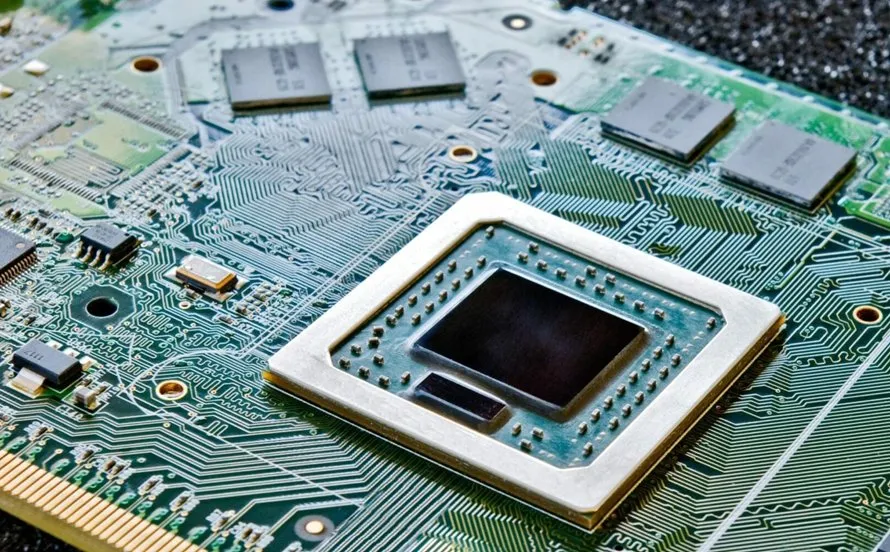
\includegraphics[width=\paperwidth,keepaspectratio]{pictures/background/background-PCB.png}}
        };
    \end{tikzpicture}
}
\begin{frame}
    \begin{multicols}{2}
        \begin{beamercolorbox}[sep=8pt,center,shadow=true,rounded=true, wd=0.5\textwidth]{title}
            {\usebeamerfont{title}Merci!\par}%
        \end{beamercolorbox}%
    \vfill\null
    \columnbreak
    \end{multicols}
\end{frame}


% VOTE
\usebackgroundtemplate{
\begin{tikzpicture}[remember picture, overlay]
        \node[at=(current page.center)] {
            {
\includegraphics[width=\paperwidth,keepaspectratio]{pictures/background/background-pcb-poster.png}}
        };
    \end{tikzpicture}
}

\begin{frame}
    \centering
    \Large

    \textcolor{white}{\LARGE{\textbf{Vote sur le prochain PPPPP}}}\\
    \vspace{24pt}

    \only<1> {
        \textcolor{white}{
        \LARGE{\textbf{Deep-Dive sur les composantes Passives}}}\\

        \begin{itemize}
            \item \textcolor{white}{Types de condensateurs}
            \item \textcolor{white}{Derating de condensateurs}
            \item \textcolor{white}{Courbes d'impédance}
            \item \textcolor{white}{Saturation de bobines}
            \item \textcolor{white}{Normes et spécifications}
            \item \textcolor{white}{Comment choisir une composante}
        \end{itemize}
    }
    \only<2> {
        \textcolor{white}{
        \LARGE{\textbf{Bonnes pratiques de Schéma \& Layout}}}\\

        \begin{itemize}
            \item \textcolor{white}{Quoi mettre sur un silkscreen}
            \item \textcolor{white}{Notes sur un schéma}
            \item \textcolor{white}{Protections de circuit}
            \item \textcolor{white}{Comment utiliser les couches mécaniques}
            \item \textcolor{white}{Comment bien faire un BOM}
        \end{itemize}
    }
    \only<3> {
        \textcolor{white}{
        \LARGE{\textbf{Comment se déplace un signal sur un PCB}}}\\

        \begin{itemize}
            \item \textcolor{white}{Où l'impédance est la plus faible?}
            \item \textcolor{white}{Retour de courant}
            \item \textcolor{white}{Ground Bounce}
            \item \textcolor{white}{Vitesse de déplacement d'un signal}
            \item \textcolor{white}{Tout est une ligne de transmission}
        \end{itemize}
    }

    \only<4> {
        \begin{itemize}
            \item \textcolor{white}{\LARGE{\textbf{Deep-Dive sur les composantes Passives}}}
            \bigskip
            \item \textcolor{white}{\LARGE{\textbf{Bonnes pratiques de Schéma \& Layout}}}
            \bigskip
            \item \textcolor{white}{\LARGE{\textbf{Comment se déplace un signal sur un PCB}}}
        \end{itemize}
    }
\end{frame}


\end{document}
